\documentclass[17pt,xcolor={svgnames,rgb,dvipsnames}]{beamer}

\usepackage{StyleBeamer}

%\usetikzlibrary{patterns.meta}

%\selectcolormodel{cmyk}

%\usepackage{wrapfig}
%\makeatletter
%\setlength{\parskip}{1ex}
%\newcommand{\@minipagerestore}{\setlength{\parskip}{1ex}}

\setbeamertemplate{navigation symbols}{}

\usetikzlibrary{patterns.meta}

% Début du document
%%%%%%%%%%%%%%%%%%%
\begin{document}

\title{Questions flash}
\frame{\titlepage}

\centering
\begin{question}
Factoriser $A=(3+2x)(x-2)+(5-x)(x-2)$
\end{question}

\begin{question}
Quel est l'ensemble hachuré?

\begin{center}
\begin{tikzpicture}[scale=1.5]

\draw (-3,-2) rectangle (3,2);
\draw[fill=DarkOrange,fill opacity=0.5] (1,0) circle (1.5);
\draw[fill=DodgerBlue!50!DeepSkyBlue,fill opacity=0.5] (-1,0) circle (1.5);
\draw (1,0) circle (1.5);
\node (A) at (1.3,0) {A};
\node (B) at (-1.3,0) {B};

\clip (1,0) circle (1.5);
\draw[fill=black,pattern=north east lines,draw=none,opacity=0.75] (-1,0) circle (1.5);

\end{tikzpicture}
\end{center}

\end{question}

\begin{question}
Reproduire à la main la figure ci-dessous et représenter l'ensemble $\overline A \cup B$:

\begin{center}
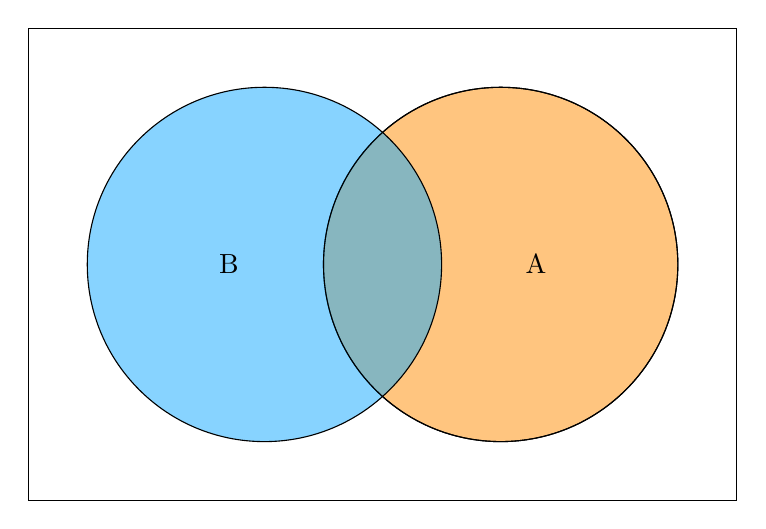
\begin{tikzpicture}[scale=1.5]

\draw (-3,-2) rectangle (3,2);
\draw[fill=DarkOrange,fill opacity=0.5] (1,0) circle (1.5);
\draw[fill=DodgerBlue!50!DeepSkyBlue,fill opacity=0.5] (-1,0) circle (1.5);
\draw (1,0) circle (1.5);
\node (A) at (1.3,0) {A};
\node (B) at (-1.3,0) {B};

%\clip (1,0) circle (1.5);
%\draw[fill=black,draw=none,opacity=0.75] (-1,0) circle (1.5);

\end{tikzpicture}
\end{center}
\end{question}

\end{document}
